\documentclass[
  a4paper,
  12pt,
]{article}
\usepackage{amsmath, amsthm, amsfonts, amssymb}
\usepackage{microtype}
\usepackage{geometry}
\usepackage{booktabs}
\usepackage{graphicx}
\usepackage{caption, subcaption}
% \usepackage{subcaption}
\usepackage{comment}

\usepackage{tikz}
\usetikzlibrary{3d, calc}

\usepackage{hyperref}
\usepackage[capitalise,nameinlink,noabbrev]{cleveref}
\usepackage{xcolor}
\hypersetup{ % this is just my personal choice, feel free to change things
  colorlinks,
  linkcolor={red!50!black},
  citecolor={blue!50!black},
  urlcolor={blue!80!black},
}
\colorlet{my_red}{red!50!black}
\colorlet{my_blue}{blue!65!black}
\colorlet{my_gold}{orange!70!black}
\colorlet{constraint_line}{my_red}
\colorlet{feasible_region}{my_blue!25}
\colorlet{vertex_point}{my_gold}
\colorlet{axis_line}{black!70}
\colorlet{axis_text}{black!85}

\usepackage{cancel}
\usepackage{mathtools}

\usepackage{enumerate}
\usepackage{enumitem}

%%% Norms and absolute values
\DeclarePairedDelimiter\abs{\lvert}{\rvert}
\DeclarePairedDelimiter\norm{\lVert}{\rVert}

%%% Sets
\DeclareMathOperator*{\conv}{conv} % Convex hull
\DeclareMathOperator*{\cone}{cone} % Conical hull
\DeclareMathOperator*{\aff}{aff}   % Affine hull

%%% Topology
\DeclareMathOperator*{\intr}{int}  % Interior
\DeclareMathOperator*{\rint}{rint} % Relative interior
\DeclareMathOperator*{\cl}{cl}     % Closure
\DeclareMathOperator*{\bd}{bd}     % Boundary
\DeclareMathOperator*{\rbd}{rbd}   % Relative boundary

%%% Convexity
\DeclareMathOperator*{\slope}{slope}  % Slope
\DeclareMathOperator*{\epi}{epi}      % Epigraph

%%% Common commands
\providecommand{\N}{\mathbb{N}}  % Natural numbers
\providecommand{\Z}{\mathbb{Z}}  % Integers
\providecommand{\Q}{\mathbb{Q}}  % Rationals
\providecommand{\R}{\mathbb{R}}  % Reals
\providecommand{\C}{\mathbb{C}}  % Complex numbers

% chktex-file 15
% chktex-file 1
% chktex-file 8

\usepackage{xparse}

\newtheoremstyle{exerciseStyle}
{ } % Space above
{ } % Space below
{\normalfont} % Body font
{ } % Indent amount
{\bfseries} % Theorem head font
{.} % Punctuation after theorem head
{ } % Space after theorem head
{\thmname{#1}\thmnumber{ #2}} % Theorem head spec (can be left empty, meaning `normal`)
\theoremstyle{exerciseStyle}
\newtheorem{exercise}{Exercise}[section]

\newtheoremstyle{solutionStyle}
{ } % Space above
{ } % Space below
{\normalfont} % Body font
{ } % Indent amount
{\bfseries} % Theorem head font
{.} % Punctuation after theorem head
{ } % Space after theorem head
{\thmname{#1}\thmnumber{ #2}} % Theorem head spec (can be left empty, meaning `normal`)
\theoremstyle{solutionStyle}
\newtheorem{solution}{Solution}[section]

\newcommand{\setexsol}[1]{%
  \setcounter{exercise}{\numexpr#1-1\relax}%
  \setcounter{solution}{\numexpr#1-1\relax}%
}

\newtheoremstyle{manualStyle}
{ }{ }{\normalfont}{ }{\bfseries}{}{ }% no punctuation here
{\thmname{#1}\thmnumber{ #2}{\normalfont\thmnote{ (#3)}}.}

\theoremstyle{manualStyle}

\makeatletter
% \DeclareManualTheorem{<shortname>}{<Printed Heading>}
% -> defines:
%    - innermanual<shortname> (the actual theorem env)
%    - manual<shortname>  (wrapper with manual number + optional note)
% tex-fmt: off
\NewDocumentCommand{\DeclareManualTheorem}{mm}{%
  \newtheorem{innermanual#1}{#2}%
  \NewDocumentEnvironment{manual#1}{m o}
  {%
    \@namedef{theinnermanual#1}{##1}%
    \IfNoValueTF{##2}%
    {%
      \begin{innermanual#1}%
    }{%
      \begin{innermanual#1}[##2]%
    }%
  }{%
    \end{innermanual#1}%
  }%
}
% tex-fmt: on
\makeatother

% Instantiate your three:
\DeclareManualTheorem{prop}{Proposition}
\DeclareManualTheorem{lemma}{Lemma}
\DeclareManualTheorem{theorem}{Theorem}
\DeclareManualTheorem{corollary}{Corollary}


\numberwithin{equation}{section}

\title{
  MAT4120\\
  \small{Mandatory assignment for Mathematical Optimization}
}
\author{August Femtehjell}
\date{\today}

\begin{document}

\maketitle

\tableofcontents

\begin{abstract}
  This document contains my solutions to the mandatory assignment for the course MAT4120--Mathematical Optimization, taught at the University of Oslo in the autumn of 2024.
  The code for everything, as well as this document, can be found at my GitHub repository: \url{https://github.com/augustfe/MAT4120}.
\end{abstract}

\setcounter{section}{2}
\setexsol{6}

\begin{exercise}
  If $S$ is convex, then $\conv(S) = S$.
  Show this!
\end{exercise}

\begin{solution}
  Since $S$ is convex, for any $u, v \in S$ and any $0 \leq \lambda \leq 1$, we have $\lambda u + (1 - \lambda) v \in S$.
  By the definition of convex hull, $\conv(S)$ is the smallest convex set containing $S$.
  Since $S$ is already convex and contains itself, it follows that $\conv(S) = S$.
\end{solution}

\setexsol{38}

\begin{exercise}
  Prove Theorem 2.4.3.
  (%
    Hint: To prove that $\rint(C)$ is convex, use Theorem 2.4.2.
    Concerning $\intr(C)$, use Exercise~2.37.
    Finally, to show that $\cl(C)$ is convex, let $x, y \in \cl(C)$ and consider the two point sequences that converge to $x$ and $y$ respectively.
    Then, look at a convex combination of $x$ and $y$ and construct a suitable sequence!%
  )
\end{exercise}

\begin{solution}
  Theorem 2.4.2 states that a convex set has a ``thin boundary'', i.e., for $C \subseteq \mathbb{R}^n$ non-empty and convex, and $x_1 \in \rint(C)$, $x_2 \in \cl(C)$, we have
  \begin{equation}
    (1 - \lambda) x_1 + \lambda x_2 \in \rint(C)
  \end{equation}
  for all $0 \leq \lambda < 1$.

  Theorem 2.4.3 on the other hand states as follows:
  If $C \subseteq \mathbb{R}^n$ is a convex set, then all sets $\rint(C)$, $\intr(C)$ and $\cl(C)$ are convex.
  Therefore, assume $C \subseteq \mathbb{R}^n$ is convex.

  Let $x, y \in \rint(C)$.
  As $\rint(C) \subseteq C \subseteq \cl(C)$, we can simply apply Theorem 2.4.2 to show that $\rint(C)$ is convex.
  By Exercise~2.37, we have that either $\intr(C) = \rint(C)$ or $\intr(C) = \emptyset$.
  In both cases, $\intr(C)$ is convex.

  Finally, let $x, y \in \cl(C)$,
  and let $x^k, y^k \in C$ be sequences such that $x^k \to x$ and $y^k \to y$.
  As $C$ is convex, $(1 - \lambda) x^k + \lambda y^k \in C$ for all $0 \leq \lambda \leq 1$, which converges to $(1 - \lambda) x + \lambda y$.
  Thus, $(1 - \lambda) x + \lambda y \in \cl(C)$, showing that $\cl(C)$ is convex.
\end{solution}

\setcounter{section}{3}
\setexsol{6}

\begin{exercise}
  Let $L$ be a line in $\mathbb{R}^n$.
  Find the nearest point in $L$ to a point $x \in \mathbb{R}^n$.
  Use your result to find the nearest point on the line $L = \{ (x, y) : x + 3y = 5 \}$ to the point $(1, 2)$.
\end{exercise}

\begin{solution}
  Let $L$ be the defined by the line $\{ b + t d : t \in \mathbb{R} \}$, where $b$ is a point on the line and $d$ is a direction vector.
  The nearest point on $L$ to a point $x \in \mathbb{R}^n$ can be found by projecting the vector $x - b$ onto the direction vector $d$.
  The projection is given by
  \begin{equation}
    \mathrm{proj}_d (x - b) = b + \frac{(x - b)^T d}{\norm{d}^2} d.
  \end{equation}

  With $b = (5, 0)$, we note that $(1, 3)$ is orthogonal to the line, so we choose the direction vector to be $d = (-3, 1)$.
  Then, the nearest point on the line $L$ to the point $(1, 2)$ is given by
  \begin{equation}
    \begin{split}
      \mathrm{proj}_d ((1, 2) - (5, 0)) &= \mathrm{proj}_d ((-4, 2))
      = (5, 0) + \frac{(-4, 2)^T (-3, 1)}{\norm{(-3, 1)}^2} (-3, 1) \\
      &= (5, 0) + \frac{14}{10} (-3, 1)
      =\left(\frac{25}{5}, 0\right) + \left(-\frac{21}{5}, \frac{7}{5}\right) \\
      &= \left(\frac{4}{5}, \frac{7}{5}\right).
    \end{split}
  \end{equation}
  Therefore, the nearest point on the line $L$ to the point $(1, 2)$ is $\left(\frac{4}{5}, \frac{7}{5}\right)$.
\end{solution}

\setexsol{18}
\begin{exercise}
  Consider the outer description of closed convex sets given in Corollary~3.2.4.
  What is this description for each of the following sets:
  \begin{enumerate}[label = (\emph{\roman*})]
    \item $C_1 = \{ x \in \mathbb{R}^n : \norm{x} \leq 1 \}$,
    \item $C_2 = \conv(\{0, 1\}^n)$,
    \item $C_3$ is the convex hull of the points $(1,1)$, $(1,-1)$, $(-1,1)$, and $(-1,-1)$ in $\mathbb{R}^2$.
    \item $C_4$ is the convex hull of all vectors in $\mathbb{R}^n$ having components that are either $1$ or $-1$.
  \end{enumerate}
\end{exercise}

\begin{solution}
  We find the outer descriptions as follows:
  \begin{enumerate}[label = (\emph{\roman*})]
    \item The half-planes are the tangents to the unit ball, as used in a previous exercise.
    \item With $e_i$ being the $i$th standard basis vector in $\mathbb{R}^n$, the half-planes are given by $e_i^T x = 0$ and $e_i^T x = 1$ for $i = 1, \ldots, n$.
    \item Similarly, here the half-planes are given by $x_1 = 1$, $x_1 = -1$, $x_2 = 1$, and $x_2 = -1$, almost equivalently to (\emph{ii}).
    \item Again, the half-planes are given by $e_i^T x = 1$ and $e_i^T x = -1$ for $i = 1, \ldots, n$, almost equivalently to (\emph{ii}) and (\emph{iii}).
  \end{enumerate}
\end{solution}

\setcounter{section}{4}
\setexsol{17}

\begin{exercise}
  Consider a polyhedral cone $C = \{x \in \mathbb{R}^n : Ax \leq 0\}$ (where, as usual $A$ is a real $m \times n$-matrix).
  Show that $0$ is the unique vertex of $C$.
\end{exercise}

\begin{solution}
  Assume that $\rank(A) < n$.
  Then, there exists a non-zero vector $z$ such that $Az = 0$.
  As such, we have that for any $x \in C$ and any $\lambda \in \mathbb{R}$,
  \begin{align*}
    A(x + \lambda z) = Ax + \lambda Az = Ax \leq 0,
  \end{align*}
  showing that $x + \lambda z \in C$.
  Therefore, if $\rank(A) < n$, then $C$ has no vertices.
  As such, the exercise is missing information, as it is not necessarily true that $0$ is the unique vertex of $C$.

  As a simple counterexample, consider
  \begin{equation}
    C = \{ (x_0, x_1) \in \mathbb{R}^2 : x_0 \leq 0 \},
  \end{equation}
  which contains the line $\{ (0, x_1) : x_1 \in \mathbb{R} \}$, and thus has no vertices.

  If on the other hand $\rank(A) = n$, then there exists an $n \times n$ submatrix $A'$ of $A$ such that $\det(A') \neq 0$.
  Then, the only solution to $A'x = 0$ is $x = 0$, regardless of which such submatrix we choose.
  Therefore, $0$ is the only point that can be a vertex of $C$.
\end{solution}

\setexsol{22}

\begin{exercise}
  Let $P \subset \mathbb{R}^2$ be the polyhedron being the solution set of the linear system
  \begin{equation}
    \begin{array}{rcrcl}
      x & - & y & \leq & 0 \\
      -x & + & y & \leq & 1 \\
      & & 2y & \geq & 5 \\
      8x & - & y & \leq & 16 \\
      x & + & y & \geq & 4
    \end{array}
  \end{equation}
  Find all the extreme points of P.
\end{exercise}

\begin{solution}
  Written in matrix form, we have
  \begin{equation}
    A =
    \begin{bmatrix}
      1 & -1 \\
      -1 & 1 \\
      0 & -2 \\
      8 & -1 \\
      -1 & -1
    \end{bmatrix}
    \quad\text{and}\quad
    b =
    \begin{bmatrix}
      0 \\
      1 \\
      -5 \\
      16 \\
      -4
    \end{bmatrix}.
  \end{equation}
  I chose to solve this using Python, with the library SymPy.
  The code is freely available at \href{https://github.com/augustfe/MAT4120/blob/main/mandatory/extreme_points.py}{\texttt{mandatory/extreme\_points.py}}, and briefly works by iterating over all $2 \times 2$ submatrices of $A$ and checking if the corresponding equations yield a point in the feasible region.
  With this approach I found the extreme points to be
  \begin{equation}
    \left\{
      \frac{1}{2}
      \begin{bmatrix} 3 \\ 5
      \end{bmatrix},
      \frac{1}{7}
      \begin{bmatrix} 17 \\ 24
      \end{bmatrix},
      \frac{1}{16}
      \begin{bmatrix} 37 \\ 40
      \end{bmatrix}
    \right\}.
  \end{equation}
  The feasible region and all extreme points are illustrated in \cref{fig:exercise422-feasible-region}.

  \begin{figure}[h]
    \centering
    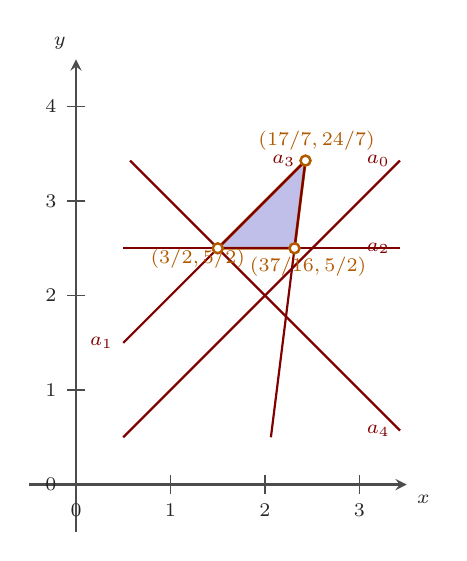
\begin{tikzpicture}[
    scale=1.2,
    >=stealth,
    axis/.style={color=axis_line, line width=0.8pt},
    tick/.style={axis, line width=0.6pt},
    axis-label/.style={color=axis_text, font=\scriptsize},
    constraint/.style={color=constraint_line, line width=0.8pt},
    constraint-label/.style={constraint, font=\scriptsize},
    vertex-line/.style={color=vertex_point, line width=1pt},
    vertex/.style={color=vertex_point, fill=white, line width=0.9pt},
    vertex-label/.style={color=vertex_point, font=\scriptsize},
  ]
  %%%%%%%%%% Feasible region %%%%%%%%%%
  \fill[feasible_region] (3/2,5/2) -- (37/16,5/2) -- (17/7,24/7) -- cycle;
  
  %%%%%%%%%% Axis lines %%%%%%%%%%
  \draw[axis, ->] (-0.5,0) -- (3.5,0) node[axis-label, below right] {$x$};
  \draw[axis, ->] (0,-0.5) -- (0,4.5) node[axis-label, above left] {$y$};
  
  %%%%%%%%%% Axis ticks %%%%%%%%%%
  \foreach \i in {0,...,3} {
    \draw[tick] (\i,0.1) -- (\i,-0.1) node[axis-label, below] {$\i$};
  }
  \foreach \i in {0,...,4} {
    \draw[tick] (0.1,\i) -- (-0.1,\i) node[axis-label, left] {$\i$};
  }
  
  \draw[vertex-line] (3/2,5/2) -- (37/16,5/2) -- (17/7,24/7) -- cycle;
  %%%%%%%%%% Constraint lines %%%%%%%%%%
  \foreach \segment/\labeltext in {
    {(0.5000,0.5000) -- (3.4286,3.4286)}/{$a_{0}$},
    {(2.4286,3.4286) -- (0.5000,1.5000)}/{$a_{1}$},
    {(0.5000,2.5000) -- (3.4286,2.5000)}/{$a_{2}$},
    {(2.0625,0.5000) -- (2.4286,3.4286)}/{$a_{3}$},
    {(0.5714,3.4286) -- (3.4286,0.5714)}/{$a_{4}$}
  } {
    \draw[constraint] \segment node[left, constraint-label] {\labeltext};
  }
  
  \def\VertexRadius{1.5pt}
  %%%%%%%%%% Vertices %%%%%%%%%%
  \foreach \vertexpos/\labelpos/\labeltext in {
    {(3/2,5/2)}/{(1.2882,2.3871)}/{$(3/2, 5/2)$},
    {(37/16,5/2)}/{(2.4565,2.3080)}/{$(37/16, 5/2)$},
    {(17/7,24/7)}/{(2.5462,3.6377)}/{$(17/7, 24/7)$}
  } {
    \filldraw[vertex] \vertexpos circle (\VertexRadius);
    \node[vertex-label] at \labelpos {\labeltext};
  }
  
\end{tikzpicture}

    \caption{Feasible region of Exercise~4.22 with the constraint boundaries and extreme points.}\label{fig:exercise422-feasible-region}
  \end{figure}
\end{solution}

\setcounter{section}{5}
\setexsol{10}

\begin{exercise}
  By the result above we have that if $f$ and $g$ are convex functions, then the function $\max\{f,g\}$ is also convex.
  Prove this result directly from the definition of a convex function.
\end{exercise}

\begin{solution}
  Let $f, g : \mathbb{R}^n \to \mathbb{R}$ be convex functions, and define $h(x) = \max\{f(x), g(x)\}$.
  Then, for any $x, y \in \mathbb{R}^n$ and any $0 \leq \lambda \leq 1$, we have
  \begin{align*}
    h(\lambda x + (1 - \lambda) y)
    &= \max\{f(\lambda x + (1 - \lambda) y), g(\lambda x + (1 - \lambda) y)\} \\
    &\leq \max\{\lambda f(x) + (1 - \lambda) f(y), \lambda g(x) + (1 - \lambda) g(y)\} \\
    &\leq \lambda \max\{f(x), g(x)\} + (1 - \lambda) \max\{f(y), g(y)\} \\
    &= \lambda h(x) + (1 - \lambda) h(y),
  \end{align*}
  showing that $h$ is convex.
\end{solution}

\setexsol{22}

\begin{manualprop}{5.1.2}[Increasing slopes]\label{prop:increasing-slopes}
  A function $f : \mathbb{R} \to \mathbb{R}$ is convex if and only if for each $x_0 \in \mathbb{R}$ the slope function
  \begin{equation}
    x \mapsto \frac{f(x)-f(x_0)}{x-x_0}
  \end{equation}
  is increasing on $\mathbb{R} \setminus \{x_0\}$.
\end{manualprop}

\begin{exercise}
  Let $f : (0, \infty) \to \mathbb{R}$ and define the function $g : (0, \infty) \to \mathbb{R}$ by $g(x) = x f(\frac{1}{x})$.
  Prove that $f$ is convex if and only if $g$ is convex.
  Hint: Prove that
  \begin{equation}
    \frac{g(x) - g(x_0)}{x - x_0} = f(\tfrac{1}{x_0}) - \frac{1}{x_0} \cdot \frac{f(\frac{1}{x}) - f(\frac{1}{x_0})}{\frac{1}{x} - \frac{1}{x_0}}
    \label{eq:exercise522-hint}
  \end{equation}
  and use \cref{prop:increasing-slopes}.
  Why is the function $x \mapsto x e^{1/x}$ convex?
\end{exercise}

\begin{solution}
  We have that
  \begin{align*}
    \frac{g(x) - g(x_0)}{x - x_0}
    &= \frac{x f(\frac{1}{x}) - x_0 f(\frac{1}{x_0})}{x - x_0} \\
    &= \frac{x f(\frac{1}{x}) - x f(\frac{1}{x_0}) + x f(\frac{1}{x_0}) - x_0 f(\frac{1}{x_0})}{x - x_0} \\
    &= \frac{x (f(\frac{1}{x}) - f(\frac{1}{x_0}))}{x - x_0} + \frac{(x - x_0) f(\frac{1}{x_0})}{x - x_0} \\
    &= f(\tfrac{1}{x_0}) + \frac{x (f(\frac{1}{x}) - f(\frac{1}{x_0}))}{x - x_0} \\
    &= f(\tfrac{1}{x_0}) + \frac{1}{x_0} \frac{x x_0 (f(\frac{1}{x}) - f(\frac{1}{x_0}))}{x - x_0}.
  \end{align*}
  Then, as
  \begin{equation*}
    \frac{x x_0}{x - x_0}
    = \frac{1}{\frac{x}{x x_0} - \frac{x_0}{x x_0}}
    = \frac{1}{\frac{1}{x_0} - \frac{1}{x}},
  \end{equation*}
  \cref{eq:exercise522-hint} follows.

  Assume $f$ is convex.
  Let $h$ be the slope function of $f$ at $x_0$, i.e.,
  \begin{equation}
    h(x) = \frac{f(x) - f(x_0)}{x - x_0}.
  \end{equation}
  As $1/x$ decreases as $x$ increases, we have that $h(1/x)$ is decreasing.
  Therefore, $-h(1/x)$ is increasing, and offsetting this with the constant $f(1/x_0)$ maintains the increasing property.
  Thus, by \cref{prop:increasing-slopes}, $g$ is convex, as it's slope function is increasing.

  With $f(x) = e^x$, we have $g(x) = x f(1/x) = x e^{1/x}$, which is therefore convex, as $e^x$ is convex.
\end{solution}

\end{document} % chktex 17
